\documentclass[titlepage]{article}
\usepackage[draft=false, cachedir=minted_cache]{minted}
\usepackage{enumitem}
\usepackage{graphicx}
\graphicspath{ {./img/} }
\usepackage[margin=.5in]{geometry} %used to set the margins
\setcounter{secnumdepth}{0} %used to get rid of section numbers
\title{
    Project 1 - Hashing \\
    CSCI 230 T Th 11:10 am \\
    Compiler: g++ \\
    OS: Linux
    }

\author{Michael Morikawa}
\date{\today}


\begin{document}
\maketitle

\section{Notes}
\subsection{Status}
I have completed all parts for separate chaining, linear probring, 
and double hashing. 
\subsection{Extra Credit}
 The second option for extra credit is pretty much fully implemented 
 however I was unable to take into account wrap around for open 
 addressing.
\subsection{Design Decisions}
I was unable to fully make use of inheritance and have all 
three hash tables be derrived from the same class. This 
is because of the different structure for separate chainging 
and open addressing. The iterators for the two types are different
 and thus can't be inherited. I was able to derive the double hashing 
 scheme from the base class which implemented linear probing.

 I also did not throw an exception for when trying to delete an 
 element that was not in the table. It simple counts probes and 
 moves on. There is also nothing to stop someone from using 
 too high of a load factor. I haven't tested it but I 
 think it would go in an infinite loop for open addressing.

 \newpage

 \section{Data}
 \textbf{Tests all done with p1large.txt}
\vspace{5mm}

\begin{tabular}{ |c|c|c|c|c| } 
\hline
\multicolumn{5}{|c|}{Hash Table Size(All Schemes)}\\
\hline
Load Factor & 0.25 & 0.5 & 0.75 & 0.9 \\
\hline
Table Size & 12799 & 6397 & 4271 & 3557 \\
\hline
\end{tabular}


\subsection{Separate Chaining}
\begin{tabular}{ |c|c|c|c|c| } 
\hline
\multicolumn{5}{|c|}{Probe and Cluster Data}\\
\hline
Load Factor & 0.25 & 0.5 & 0.75 & 0.9 \\
\hline
Avg Probes & 1.011 & 1.043 & 1.221 & 1.249\\
\hline
Max Probes & 2 & 3 & 3 & 4 \\
\hline
Total Clusters & 35 & 126 & 659 & 659\\
\hline
Avg Cluster Size & 2 & 2.048 & 2.036 & 2.102\\
\hline
Max Cluster Size & 2 & 3 & 3 & 4 \\
\hline
\end{tabular}

\subsection{Linear Probing}
\begin{tabular}{ |c|c|c|c|c| } 
\hline
\multicolumn{5}{|c|}{Probe and Cluster Data}\\
\hline
Load Factor & 0.25 & 0.5 & 0.75 & 0.9 \\
\hline
Avg Probes & 1.408 & 2.469 & 11.198 & 76.423\\
\hline
Max Probes & 2 & 3 & 3 & 4 \\
\hline
Total Clusters & 74 & 78 & 53 & 10\\
\hline
Avg Cluster Size & 5.770 & 23.346 & 47.604 & 298.8\\
\hline
Max Cluster Size & 164 & 346 & 572 & 2887 \\
\hline
\end{tabular}

\subsection{Double Hashing}
\begin{tabular}{ |c|c|c|c|c| } 
\hline
\multicolumn{5}{|c|}{Probe and Cluster Data}\\
\hline
Load Factor & 0.25 & 0.5 & 0.75 & 0.9 \\
\hline
Avg Probes & 1.024 & 1.120 & 2.073 & 3.138\\
\hline
Max Probes & 5 & 9 & 15 & 185 \\
\hline
Total Clusters & 74 & 111 & 395 & 183\\
\hline
Avg Cluster Size & 5.068 & 14.973 & 6.615 & 16.568\\
\hline
Max Cluster Size & 124 & 193 & 154 & 423 \\
\hline
\end{tabular}
\subsection{Conclusions}
From the data we see that separate chaining has the lowest average probe 
count, followed by double hashing with linear probing coming in last. This 
supports the assumption that it would perform the worst due to the clustering 
linear probing causes. For low load factors double hashing is similar to 
separate chaining for probes but as the load factor increases past 0.5 it 
becomes noticibly worse than separate chaining. The average and max clusters 
for linear probing is also the highest which is what is expected. The total 
clusters for separate chaining is higher than double hashing for a load factor 
greater than 0.5. However despite the high cluster count the cluster sizes remain 
small so the performace doesn't take as much of a hit as double hashing which has 
much larger cluster sizes.

 \newpage

\section{Source Code}
\subsection{main.cpp}
\inputminted{c++}{../../src/main.cpp}
\subsection{HashCode.hpp}
\inputminted{c++}{../../include/HashCode.hpp}
\subsection{Entry.hpp}
\inputminted{c++}{../../include/Entry.hpp}
\subsection{ChainHashMap.hpp}
\inputminted{c++}{../../include/ChainHashMap.hpp}
\subsection{OpenAddressMap.hpp}
\inputminted{c++}{../../include/OpenAddressMap.hpp}

\section{Output}

\subsection{Small Input File Tests}
\subsubsection{Separate Chaining}

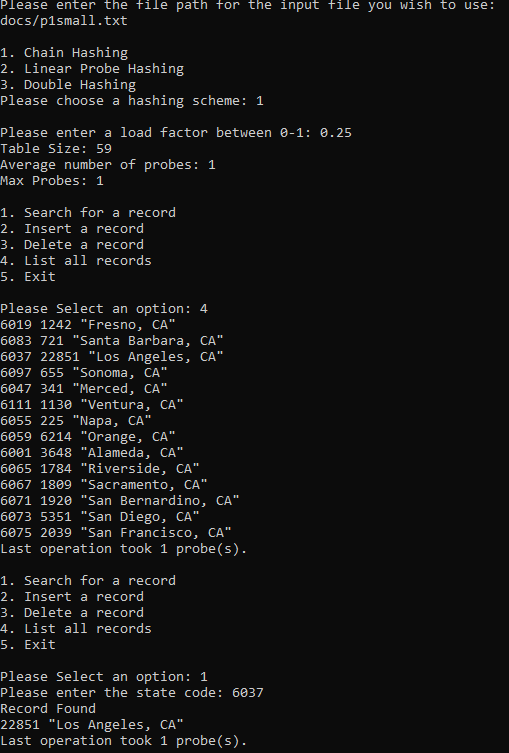
\includegraphics[]{Small_Input/LF_0_25/ChainHash_1.png}   \newpage
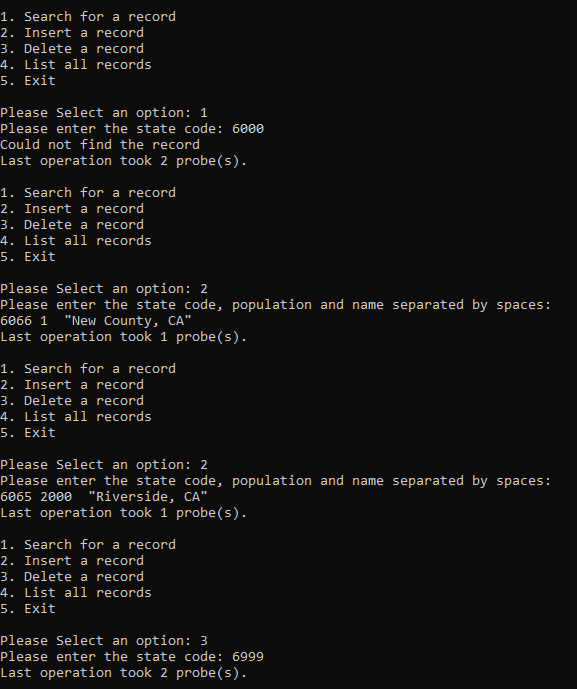
\includegraphics[]{Small_Input/LF_0_25/ChainHash_2.png}   \newpage
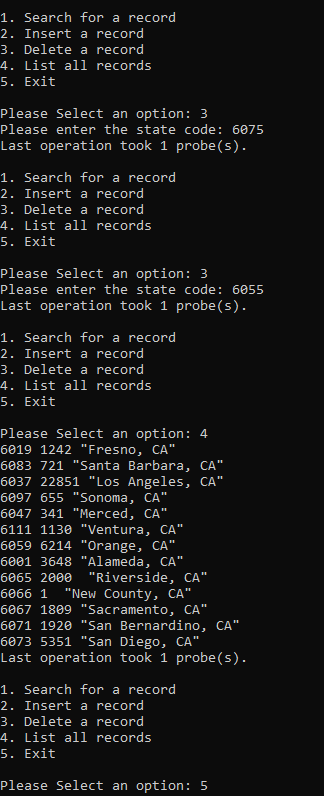
\includegraphics[]{Small_Input/LF_0_25/ChainHash_3.png}   \newpage
\subsubsection{Linear Probing}

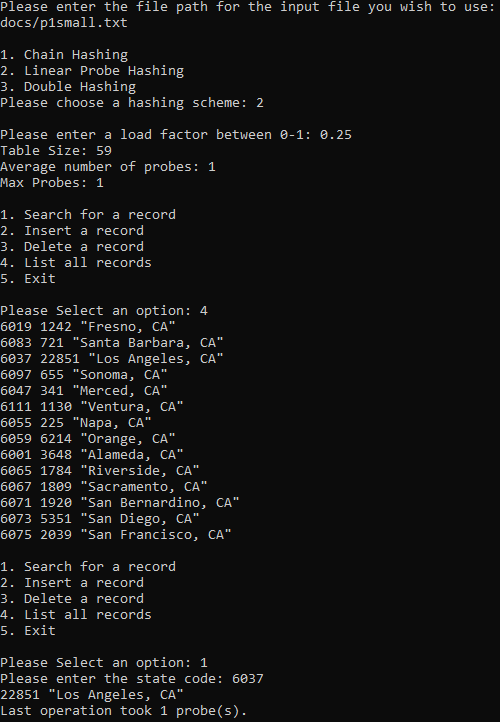
\includegraphics[]{Small_Input/LF_0_25/LinearProbe_1.png} \newpage
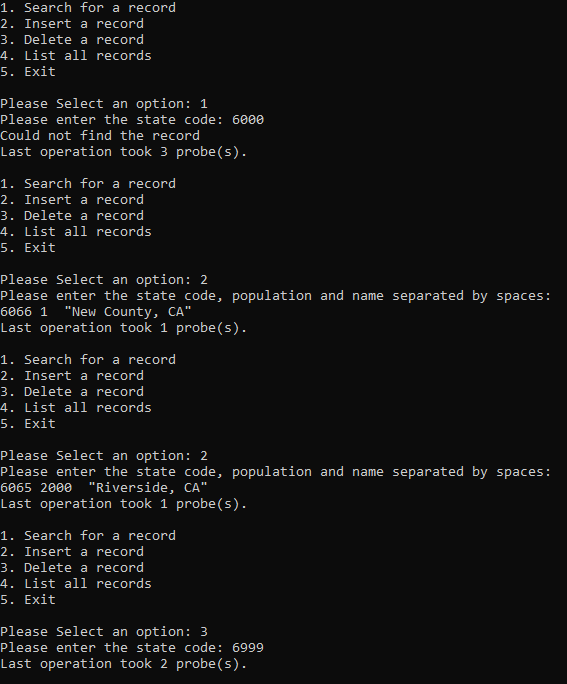
\includegraphics[]{Small_Input/LF_0_25/LinearProbe_2.png}\newpage 
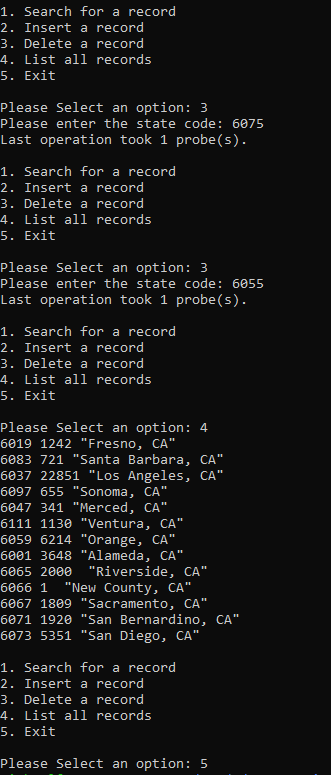
\includegraphics[]{Small_Input/LF_0_25/LinearProbe_3.png}\newpage 
\subsubsection{Double Hashing}

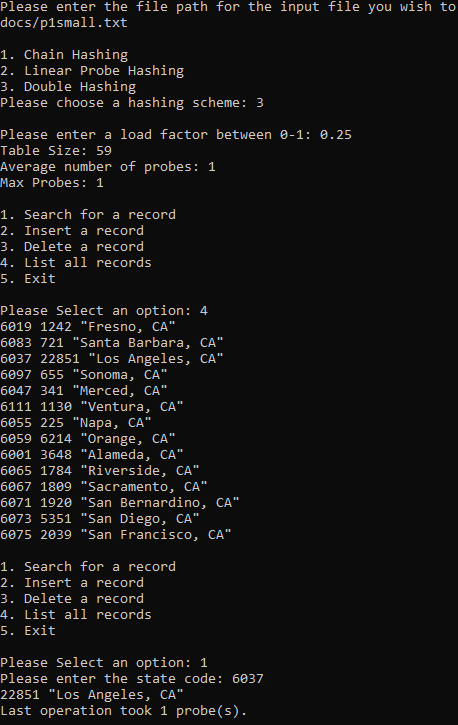
\includegraphics[]{Small_Input/LF_0_25/DoubleHash_1.png} \newpage
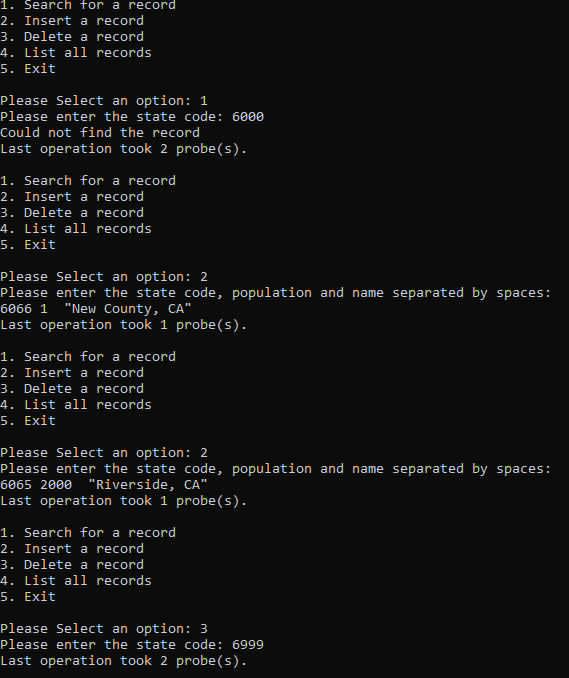
\includegraphics[]{Small_Input/LF_0_25/DoubleHash_2.png} \newpage
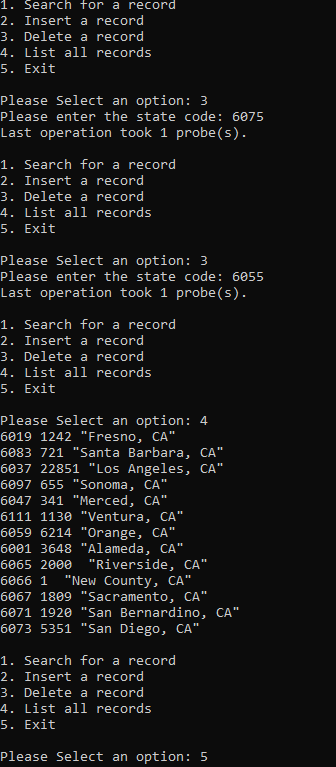
\includegraphics[]{Small_Input/LF_0_25/DoubleHash_3.png} \newpage

\subsection{Large File Probe Testing}
\subsubsection{Separate Chaining}
\subsubsection{Loadfactor = 0.25}
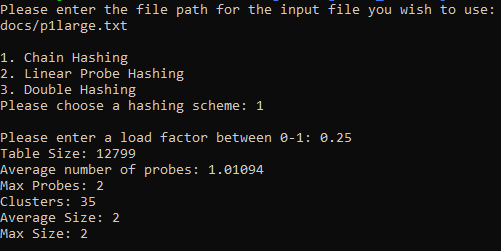
\includegraphics[]{Large_Input/LF_0_25/ChainHash.png}
\subsubsection{Loadfactor = 0.50}
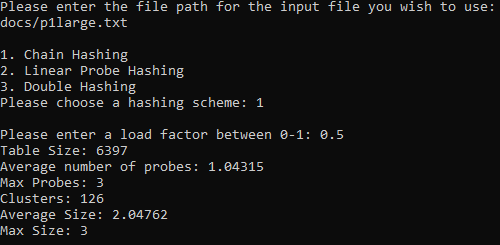
\includegraphics[]{Large_Input/LF_0_50/ChainHash.png}
\subsubsection{Loadfactor = 0.75}
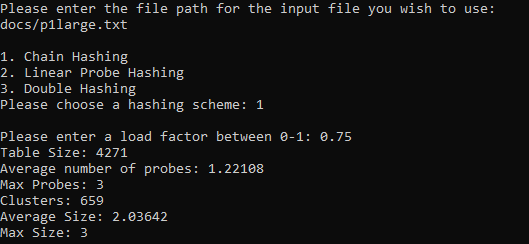
\includegraphics[]{Large_Input/LF_0_75/ChainHash.png}
\subsubsection{Loadfactor = 0.90}
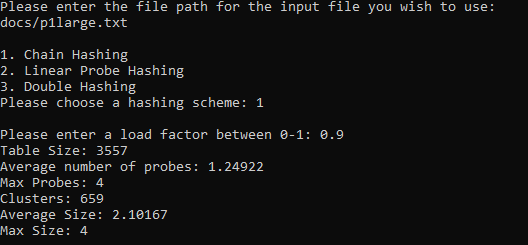
\includegraphics[]{Large_Input/LF_0_90/ChainHash.png}

\subsubsection{Linaer Probing}
\subsubsection{Loadfactor = 0.25}
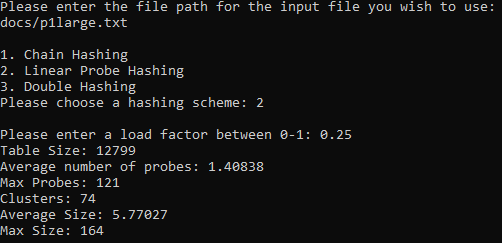
\includegraphics[]{Large_Input/LF_0_25/LinearProbe.png}
\subsubsection{Loadfactor = 0.50}
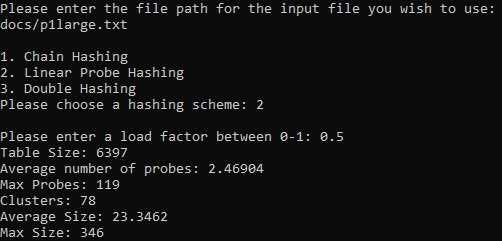
\includegraphics[]{Large_Input/LF_0_50/LinearProbe.png}
\subsubsection{Loadfactor = 0.75}
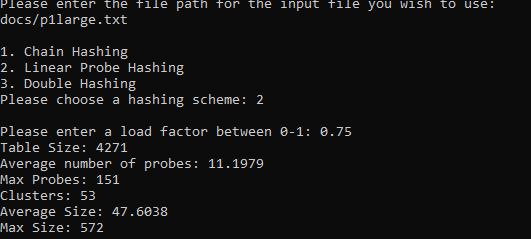
\includegraphics[]{Large_Input/LF_0_75/LinearProbe.png}
\subsubsection{Loadfactor = 0.90}
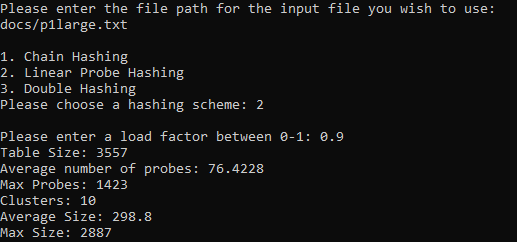
\includegraphics[]{Large_Input/LF_0_90/LinearProbe.png}

\subsubsection{Double Hashing}
\subsubsection{Loadfactor = 0.25}
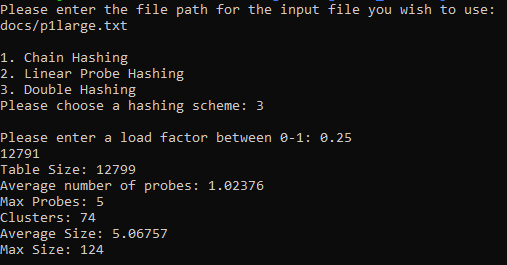
\includegraphics[]{Large_Input/LF_0_25/DoubleHash.png}
\subsubsection{Loadfactor = 0.50}
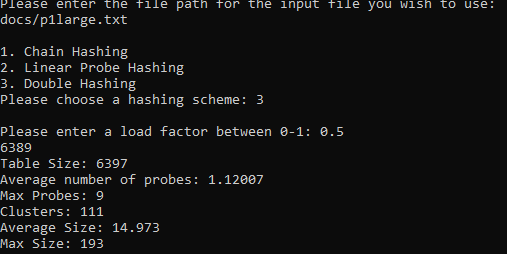
\includegraphics[]{Large_Input/LF_0_50/DoubleHash.png}
\subsubsection{Loadfactor = 0.75}
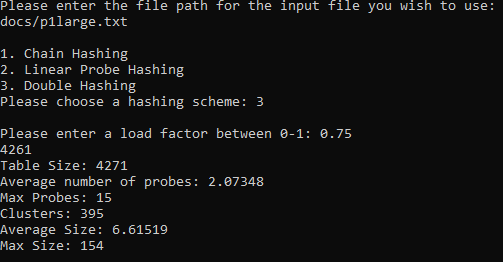
\includegraphics[]{Large_Input/LF_0_75/DoubleHash.png}
\subsubsection{Loadfactor = 0.90}
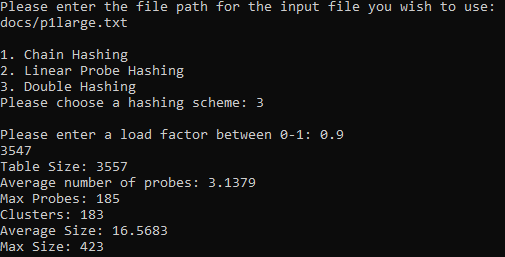
\includegraphics[]{Large_Input/LF_0_90/DoubleHash.png}
\end{document}